\section{Conditional Expectation}

  Conditional expectation is extremely important, especially in the context of stochastic processes, which is talked about in more detail in another set of notes. 

  First, note that when we talk about the probability of event $A$ happening, or equivalently, the probability of $\omega \in A$, we can write this as the expected value of the indicator function $A$. 
  \begin{equation}
    \mathbb{P}(A) = \mathbb{E}[1_A]
  \end{equation}
  This will come in handy later in connecting conditional probability and expectation. 

  Now conditional expectation is quite tricky to understand at first. We will start by defining it given a $\sigma$-algebra and then given a random variable. 

  \begin{definition}[Conditional Expectation]
    Given a probability space $(\Omega, \mathcal{F}, \mathbb{P})$, a sub-$\sigma$-algebra $\mathcal{G} \subset \mathcal{F}$, and an $\mathcal{F}$-measurable random variable $X$ (with $\mathbb{E}[X] < \infty$), the \textbf{conditional expectation of $X$ given $\mathcal{G}$} is defined to be the $\mathcal{G}$-measurable random variable $Y = \mathbb{E}[X \mid \mathcal{G}]$ satisfying 
    \begin{equation}
      \int_A X \,d\mathbb{P} = \int_A Y \,d \mathbb{P}
    \end{equation}
    or equivalently, 
    \begin{equation}
      \mathbb{E}[X \cdot 1_A] = \mathbb{E}[Y \cdot 1_A]
    \end{equation}
    for all $A \in \mathcal{G}$. Any $Y$ satisfying these two conditions is said to be a \textbf{version} of $\mathbb{E}[X \mid \mathcal{F}]$. The critical detail to note here is that the conditional expectation $Y$, has the same expected value as $X$ does, not over just the whole $\mathcal{G}$, but \textit{in every subset $G$ of $\mathcal{G}$}. 
  \end{definition}

  We state without proof that $\mathbb{E}[X \mid \mathcal{G}]$ exists and is almost surely unique. For now, we can interpret this as the best approximation of the $\mathcal{F}$-measurable $X$ with the $\mathcal{G}$-measurable $Y$. Here is a useful analogy. Say that we have some "fine" function $X$ defined on the interval $[0, 1]$ with a fine Borel $\sigma$-algebra $\mathcal{F}$. 
  \begin{enumerate}
    \item If we are given some sub-$\sigma$-algebra $\mathcal{G}$ composed of $\emptyset, [0, 0.5], (0.5, 1], [0, 1]$, then $Y$ would be the step function defined constantly on these intervals. 
    \item If we are given a finer sub-$\sigma$-algebra $\mathcal{H}$ generated by $[0, 0.25), [0.25, 0.5), [0.5, 0.75), [0.75, 1]$, then this would give a $\mathcal{H}$-measurable function that is a better approximation of $X$. 
  \end{enumerate}
  \begin{center}
    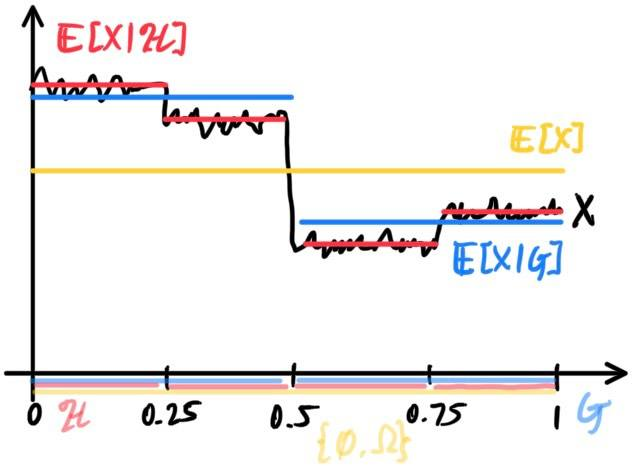
\includegraphics[scale=0.33]{img/function_approximation_conditional.jpg}
  \end{center}

  Therefore, we can see that if $\mathbb{E}[X \mid \mathcal{G}]$ is $\mathcal{F}$-measurable, then 
  \begin{equation}
    X = \mathbb{E}[X \mid \mathcal{G}]
  \end{equation}
  since its value coincides with $X$ for every event in $\mathcal{F}$. One way to think about it is that $\mathbb{E}[X \mid \mathcal{G}]$ is the conditional expectation of $X$ (which is "detailed" up to resolution $\sigma(\mathcal{G})$) taken with a camera of resolution $\mathcal{G}$. The finer (bigger) the $\sigma$-algebra is, the higher the resolution. 

\subsection{Properties of Conditional Expectation}

  \begin{theorem}[Tower Rule]
    The expectation of $X$ and its approximation always coincides. 
    \begin{equation}
      \mathbb{E}[X] = \mathbb{E}[\mathbb{E}[X \mid \mathcal{G}]]
    \end{equation}
  \end{theorem}

  \begin{lemma}
    Let $\mathbb{E}[|X|] , \mathbb{E}[|Y|] < \infty$. Then, 
    \begin{enumerate}
      \item Conditional expectation is linear
      \begin{equation}
        \mathbb{E}[a X + b Y \mid \mathcal{G}] = a \mathbb{E}[X \mid \mathcal{G}] + b \mathbb{E}[Y \mid \mathcal{G}]
      \end{equation}
      
      \item If $X \leq Y$, then 
      \begin{equation}
        \mathbb{E}[X \mid \mathcal{G}] \leq \mathbb{E}[Y \mid \mathcal{G}]
      \end{equation}
    \end{enumerate}
  \end{lemma}

  \begin{theorem}[Jensen's Inequality]
    If $\varphi$ is convex and $\mathbb{E}[|X|], \mathbb{E}[|\varphi(X)|] < \infty$, then 
    \begin{equation}
      \varphi(\mathbb{E}[X \mid \mathcal{G}]) \leq \mathbb{E}[\varphi(X) \mid \mathcal{G}]
    \end{equation}
  \end{theorem}

  \begin{theorem}
    Conditional expectation is a contraction in $L^p$, $p \geq 1$. 
  \end{theorem}

  \begin{theorem}
    If $X$ is $\mathcal{F}$-measurable and $\mathbb{E}[|Y|], \mathbb{E}[|XY|] < \infty$, then 
    \begin{equation}
      \mathbb{E}[XY \mid \mathcal{F}] = X \mathbb{E}[Y \mid \mathcal{F}]
    \end{equation}
  \end{theorem}

  \begin{theorem}
    Suppose $\mathbb{E}[X^2] < \infty$. Then, $\mathbb{E}[X \mid \mathcal{G}]$ is the $\mathcal{G}$-measurable function $Y$ that minimizes the mean squared error 
    \begin{equation}
      \mathbb{E}[ (X - Y)^2]
    \end{equation}
  \end{theorem}

  This gives a nice geometric interpretation of $\mathbb{E}[X \mid \mathcal{G}]$. Given that $X$ lives in the Hilbert space $L^2_\mathcal{F} (\Omega)$, $\mathbb{E}[X \mid \mathcal{G}]$ is the projection of $X$ onto the subspace $L^2_\mathcal{G} (\Omega)$. 
  \begin{center}
    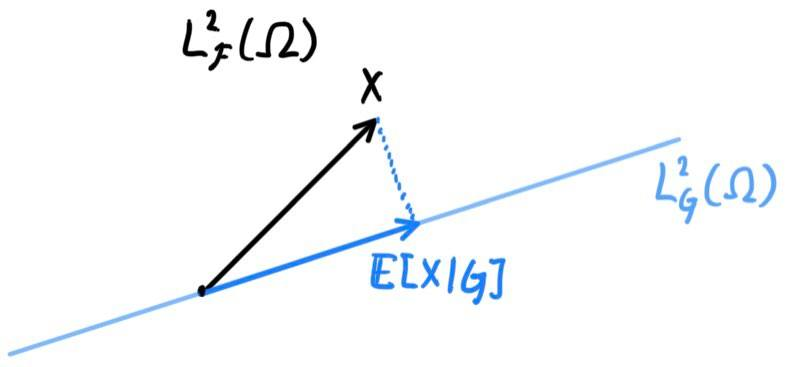
\includegraphics[scale=0.3]{img/Hilbert_Space_projection.jpg}
  \end{center}
  Therefore, we can change the way think about $\mathbb{E}[X]$. It is not just a value, but rather, we can think of it as our best prediction of $X$ given no information. Specifically, 
  \begin{equation}
    \mathbb{E}[X] = \mathbb{E}[X \mid \{\emptyset, \Omega\}]
  \end{equation}
  That is, letting $\mathcal{G}$ be the trivial $\sigma$-algebra, we must find the best approximation of $X$ that is $\mathcal{G}$-measurable. But any random variable that is $\mathcal{G}$-measurable must be constant, since if we take the preimage of any singleton set $\{x\} \in \mathcal{R}$, then it must be either $\emptyset$ ($X$ does not map to it) or $\Omega$ ($X$ maps all of $\Omega$ to it).

\subsection{Perfect Information vs No Information}

  Now let us state some properties on how certain $\sigma$-algebras can change the conditional expectation of certain random variables. 

  \begin{theorem}[Perfect Information]
    If $X$ is $\mathcal{G}$-measurable, then 
    \begin{equation}
      \mathbb{E}[X \mid \mathcal{G}] = X
    \end{equation}
    That is, the values of $X$ are defined on $\sigma(X) \subset \mathcal{F}$ and so has a detail level of $\sigma(X)$. But if we condition it on an even finer $\mathcal{G} \supset \sigma(X)$, then we are taking a picture of $X$ with something that has overly high resolution, and so our best approximation of $X$ is $X$ itself. Indeed, if $X$ lives in $L_\mathcal{G} (\Omega)$, then its projection onto $L_\mathcal{G} (\Omega)$ is $X$ itself. 
  \end{theorem}

  \begin{theorem}[Irrelevant Information]
    If $X$ is independent of $\mathcal{G}$, i.e. $\sigma(X)$ and $\mathcal{G}$ are independent $\sigma$-algebras, then 
    \begin{equation}
      \mathbb{E}[X \mid \mathcal{G}] = \mathbb{E}[X]
    \end{equation}
    That is, our best approximation of $X$ given information $\mathcal{G}$ is $\mathbb{E}[X]$ itself, i.e. if you don't know anything about $X$, then the best guess is the mean $\mathbb{E}[X]$. To see why, note that independence means that for all $A \in \mathcal{G}$ and $B \in \mathcal{R}$, 
    \begin{equation}
      \mathbb{P}(X^{-1} (B) \cap A) = \mathbb{P}(X^{-1}(B)) \cdot \mathbb{P}(A)
    \end{equation}
  \end{theorem}

  \begin{theorem}[Trivial Information]
    If $\mathcal{G} = \{\emptyset, \Omega\}$, then 
    \begin{equation}
      \mathbb{E}[X \mid \mathcal{G}] = \mathbb{E}[X]
    \end{equation}
    This makes sense since we're trying to measure $\sigma(X)$-measurable $X$ with the trivial $\mathcal{G}$, and the only function that is measurable w.r.t. the trivial $\sigma$-algebra is a constant function (since the preimage of every Borel set in $\mathcal{R}$ must be either $\Omega$ or $\emptyset$). This is the same as projecting $X$ to the line of constant functions in $L_\mathcal{F}(\Omega)$. 
  \end{theorem}

  \begin{theorem}
    If $\mathcal{F}_1 \subset \mathcal{F}_2$, then 
    \begin{enumerate}
      \item $\mathbb{E}[ \mathbb{E}[X \mid \mathcal{F}_1] \mid \mathcal{F}_2] = \mathbb{E}[X \mid \mathcal{F}_1]$. 
      \item $\mathbb{E}[ \mathbb{E}[X \mid \mathcal{F}_2] \mid \mathcal{F}_1] = \mathbb{E}[X \mid \mathcal{F}_1]$. 
    \end{enumerate}
    In other words, the smaller $\sigma$-algebra always wins. 
  \end{theorem}

  We can see this visually since in both cases, we are projecting $X$ onto $L^2_{\mathcal{F}_1} (\Omega)$ and onto $L^2_{\mathcal{F}_2} (\Omega)$, but either way, we end up in $L^2_{\mathcal{F}_1} (\Omega)$. Additionally, this is also consistent with our camera analogy, where $\mathbb{E}[X \mid \mathcal{G}]$ is like taking a picture of random variable $X$ with a camera of resolution $\mathcal{G}$. Conditional expectation is essentially an averaging/blurring operator. So, $\mathbb{E}[\mathbb{E}[X \mid \mathcal{G}] \mid \mathcal{H}]$ is like taking a picture of $X$ with resolution $\mathcal{H}$ and then with $\mathcal{G}$. The lower resolution would always win. 

\subsection{Computation of Conditional Expectation}

  \begin{definition}
    Given probability space $(\Omega, \mathcal{F}, \mathbb{P})$, the conditional expectation of $Y$ given $X$ is the random variable 
    \begin{equation}
      \mathbb{E}[X \mid Y] \coloneqq \mathbb{E}[X \mid \sigma(Y)]
    \end{equation}
    Note that since both $X$ and $Y$ are random variables, they are both $\mathcal{F}$-measurable. However, this doesn't mean that they may be $\mathcal{G}$-measurable for some sub-$\sigma$-algebra $\mathcal{G}$. So, as long as $\sigma(Y) \subset \sigma(X)$ (neither of which may be $\mathcal{F}$), we have some nontrivial approximation. 
  \end{definition}

  Now let's introduce a new way to think about expectation and conditional expectation in general. 
  \begin{enumerate}
    \item The first step is to think of $\mathbb{E}[X]$ not as a value $\mu$ but as the best estimate for the value of a random variable $X$ in the absence of any information. To minimize the squared error 
    \begin{equation}
      \mathbb{E}[ (X - e)^2] = \mathbb{E}[ X^2 - 2 e X + e^2] = \mathbb{E}[X^2] - 2 e \mathbb{E}[X] + e^2
    \end{equation}
    we differentiate with respect to $e$ to obtain $2e - 2 \mathbb{E}[X] = 0 \implies e = \mathbb{E}[X]$. For example, if I throw a fair die and you have to estimate its value $X$, according to the analysis above, your best bet is to guess $\mathbb{E}[X] = 3.5$ since $\Omega = \{1, 2, 3, 4, 5, 6\}$. On specific rolls of the die, this will be an over-estimate of an underestimate, but on the long run it minimizes the mean square error. 
    
    \item If we \textit{do} have additional information, then we use conditional expectation. Suppose that I tell you that $X$ is an even number. Then, I would guess that the possible values of $X$ are $\{2, 4, 6\}$, and so the our conditional expectation is $4$. Similarly, if I told you that $X$ is odd, then the conditional expectation is $3$. This additional information can be put into a random variable $Y: \Omega \rightarrow \mathbb{R}$ defined 
    \begin{equation}
      Y(\omega) = \begin{cases} 0 & \text{ if } \omega = 2, 4, 6 \\ 1 & \text{ if } \omega = 1, 3, 5 \end{cases}
    \end{equation}
    Then, we can say that $\mathbb{E}[X \mid Y = 0] = 4$ and $\mathbb{E}[X \mid Y = 1] = 3$. We can interpret this as the conditional expectation given the $\sigma$-algebra generated by these two sets $\{2, 4, 6\}$ and $\{1, 3, 5\}$. 
    
    \item Now, imagine that I roll the die and I tell you the parity of $X$. You should see that a single numerical response cannot cover both cases. You would respond $3$ if I tell you $X$ is odd ($Y = 1$) and $4$ if I tell you $X$ is even ($Y = 0$). A single numerical response is not enough because the particular piece of information I give you is \textit{itself random}. In fact, your response is necessarily a function of this particular piece of information, represented in our notation as 
    \begin{equation}
      g(Y) = \mathbb{E}[X \mid Y] = \begin{cases} 3 & \text{ if } Y = 1 \\ 4 & \text{ if } Y = 0 \end{cases}
    \end{equation}
    This is a function of $Y$, and it is consistent with our understanding of $\mathbb{E}[X \mid Y]$ as our "best estimate" of $X$ with random variable $Y$. 
    \begin{center}
      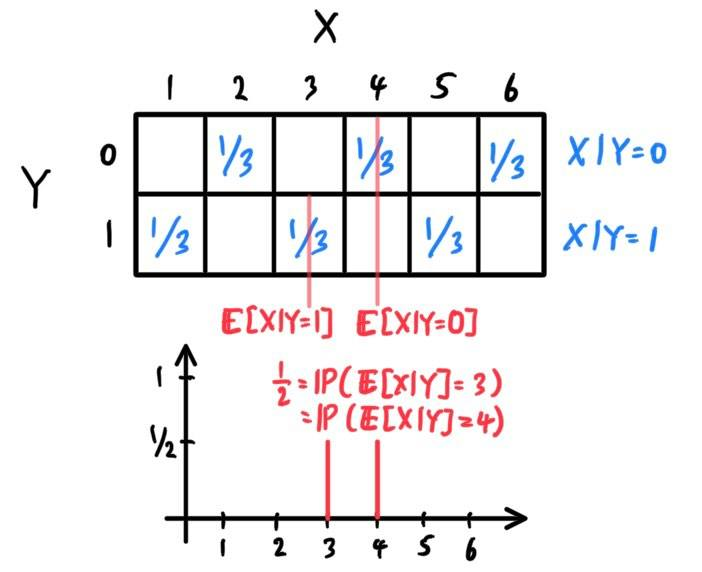
\includegraphics[scale=0.3]{img/conditional_expect_dice.jpg}
    \end{center}
  \end{enumerate}

  From the visual above, we can see that we take the joint distribution $X \times Y$, and for each value $Y = y$, we can estimate $X$ as $\mathbb{E}[X \mid Y = y]$. But now there is the additional uncertainty of what value $Y$ will take, which turns this value estimate $\mathbb{E}[X \mid Y = y]$ in a distribution $\mathbb{E}[X \mid Y]$. So, for the discrete case, 
  \begin{equation}
    \mathbb{P}\big( \mathbb{E}[X \mid Y] = \mathbb{E}[X \mid Y = y]) = \mathbb{P}(Y = y)
  \end{equation}

  Now we can talk about how to compute conditional expectation. In essence, the conditional expectation $\mathbb{E}[X \mid Y]$ is simply a function of a random variable $Y$ that is this best approximation. Given a joint random variable $(X, Y): \Omega \rightarrow \mathbb{R}^2$, we can fix a value of $Y = y$. Therefore, we are given the information that event $Y^{-1}(\{y\})$ happened, and so we can construct our conditional distribution $X \mid Y = y$, which defines a new probability measure. Taking the expectation of that gives us a number. 


  \begin{definition}[Discrete Conditional Expectation Given $Y = y$]
    Let $X, Y$ be discrete random variables, with joint random variable $(X, Y): \Omega \rightarrow \mathbb{R}^2$ and its joint PMF $p_{X, Y} (x, y)$. Recall that the conditional PMF is 
    \begin{equation}
      p_{X\mid Y}(x \mid y) \coloneqq \frac{p_{X, Y} (x, y)}{p_Y (y)}
    \end{equation}
    The \textbf{conditional expectation} of $X$ given $Y = y$ is 
    \begin{equation}
      \mathbb{E}[X \mid Y = y] = \sum_{x \in \mathcal{X}} x \, p_{X \mid Y} (x \mid y)
    \end{equation}
  \end{definition}

  \begin{definition}[Continuous Conditional Expectation Given $Y = y$]
    Let $X, Y$ be jointly continuous with joint PDF $f_{X, Y} (x, y)$. Recall that the conditional PDF is 
    \begin{equation}
      f_{X \mid Y} (x \mid y) \coloneqq \frac{f_{X, Y} (x, y)}{f_Y (y)}
    \end{equation}
    The \textbf{conditional expectation} of $X$ given $Y = y$ is 
    \begin{equation}
      \mathbb{E}[X \mid Y = y] = \int_{x \in \mathbb{R}} x \, f_{X \mid Y} (x \mid y) \, dx
    \end{equation}
    Again, we can set $\psi(y) \coloneqq \mathbb{E}[X \mid Y = y]$, which is a function of $y$ and therefore a random variable. 
  \end{definition}

  As a visual, we can take a "slice" of the joint distribution of some value of $Y$, look at the distribution of $X$ on this slice, and compute its expectation. That is, for every value of $Y = y$, there exists some (conditional) distribution of $X$ with PMF of $p_{X \mid Y} (x \mid y)$ or PDF of $f_{X \mid Y} (x \mid y)$. 
  \begin{center}
    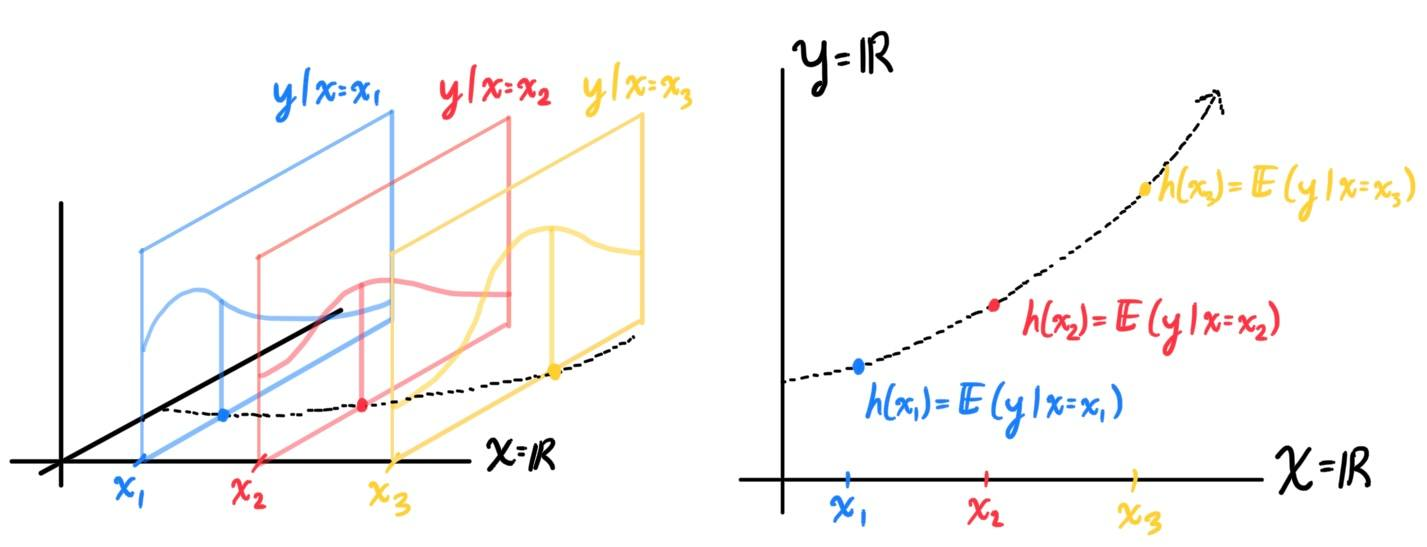
\includegraphics[scale=0.3]{img/conditional_exp.jpg}
  \end{center}
  So given a value of $Y = y$, we generally know something about $X$ (e.g. if I know humidity, I know something about the temperature) and want to find the best estimate of $X$. This is precisely the conditional expectation $\mathbb{E}[X \mid Y = y]$, and we can interpret this as a regression function $\psi(y) \coloneqq \mathbb{E}[X \mid Y = y]$, which predicts the expected value of $X$ given $Y = y$. 

  But since we don't know what exactly $Y$ is, this process is random itself, and it is only after this $Y$ is realized that we can provide the expected value of $X$. Thus, by replacing the little $y$'s with the big $Y$'s, we can construct a random variable that will estimate $X$ for us given $Y$, denoted $\mathbb{E}[X \mid Y] = \psi(Y)$. This turns out to be a $\sigma(Y)$-measurable random variable itself. 

  \begin{example}
    Let $f_{X, Y} (x, y) = \frac{1}{x}$ for $0 < y \leq x \leq 1$. Find $\mathbb{E}[Y \mid X]$. We first calculate the marginal density of $X$, which will allow us to calculate the conditional density of $Y$: 
    \begin{equation}
      f_X (x) = \int_0^x \frac{1}{x} \,dy = \frac{y}{x} \bigg|_0^x = 1 \implies f_{Y \mid X} (y \mid x) = \frac{f_{X, Y} (x, y)}{f_X (x)} = \frac{1/x}{1} = \frac{1}{x} \text{ for } 0 < y \leq x \leq 1
    \end{equation}
    Since the conditional density of $Y$ is not dependent on $x$, $Y$ is uniform from $0$ to $x$. Now calculate the expectation: 
    \begin{equation}
      \mathbb{E}[Y \mid X = x] = \int_0^x y \cdot \frac{1}{x} \,dy = \frac{x}{2}
    \end{equation}
    and so the conditional expectation is 
    \begin{equation}
      \mathbb{E}[Y \mid X] = \frac{1}{2} X
    \end{equation}
  \end{example}

  A fundamental result in statistical learning theory is that if we have two random variables $X$ and $Y$, the best predictor of $Y$ as a function of $X$ is the conditional expectation $\mathbb{E}[Y \mid X]$. 

  \begin{theorem}
    Let us have two random variables $X$ and $Y$, with $g(X) = \mathbb{E}[Y \mid X]$. Then, the function $g$ minimizes the cost function $\mathbb{E}[ (Y - h(X))^2]$. That is, 
    \begin{equation}
      \inf_{h \text{ meas.}} \mathbb{E}[( Y - h(X))^2] = \mathbb{E} [(Y - g(X))^2]
    \end{equation}
  \end{theorem}

  We restate the tower rule again. 

  \begin{theorem}[Tower Rule]
    We know that $\mathbb{E}[Y \mid X]$ is the random variable $\psi(X)$ that is a transformed version of $X$. Then, we have
    \begin{equation}
      \mathbb{E}[ \mathbb{E}[Y \mid X]] = \mathbb{E}[Y]
    \end{equation}
    This is confusing notation due to the iterated expectations, but note that the term on the inside is a transformed random variable of $X$, while the expectation on the outside computes the expectation of this transformed random variable. So, letting $\psi(X) = \mathbb{E}[Y \mid X]$, we can equivalently write 
    \begin{equation}
      \mathbb{E}[ \psi(X)] = \mathbb{E}[Y]
    \end{equation}
    Intuitively, this makes sense, since $\mathbb{E}[Y \mid X]$ is the random variable that tries to "model" $Y$ given (random) information from $X$, so its expectation must be the expectation of $Y$ itself. 
  \end{theorem}
  \begin{proof}
    We can just expand this out. We will do it for the discrete case. 
    \begin{align*}
      \mathbb{E}[ \mathbb{E}[Y \mid X]] & = \sum_x p_X (x) \, \underbrace{\mathbb{E}[Y \mid X = x]}_{\psi(x)} \\
      & = \sum_x \bigg( p_X (x) \cdot \sum_y y \cdot p_{Y \mid X} (y \mid x) \bigg) \\
      & = \sum_x \bigg( p_X (x) \cdot \sum_y y \cdot \frac{p_{X, Y} (x, y)}{p_X (x)} \\
      & = \sum_{x, y} y \cdot p_{X, Y} (x, y) \\
      & = \sum_y \bigg( y \cdot \sum_x p_{X, Y} (x, y) \bigg) \\
      & = \sum_y y \cdot p_Y (y) \\
      & = \mathbb{E}[Y]
    \end{align*}
  \end{proof}

  \begin{example}
    Consider the random sum of random variables $S_N = \sum_{i=1}^N X_i$, where $X_i$ are iid and $N$ is independent of $X_i$'s. Then, we can use the tower rule to write $\mathbb{E}[S_N] = \mathbb{E}[\mathbb{E}[S_N \mid N]]$. $\mathbb{E}[S_N \mid N]$ is a transformed random varibale of $N$, and to compute its closed form we should just compute $\mathbb{E}[S_N \mid N = n]$ and replace $n$ with $N$. 
    \begin{equation}
      \mathbb{E}[S_N \mid N = n] = \mathbb{E}[S_n] = \mathbb{E} \bigg( \sum_{i=1}^n X_i \bigg) = n \mathbb{E}[X]
    \end{equation}
    remember that $\mathbb{E}[X]$ is just a number, so replacing $n$ with $N$ gives $\mathbb{E}[S_N \mid N] = N \mathbb{E}[X]$, i.e. the random variable $N$ multiplied by $\mathbb{E}[X]$. Therefore, 
    \begin{equation}
      \mathbb{E}[\mathbb{E}[S_N \mid N]] = \mathbb{E}[N \mathbb{E}[X]] = \mathbb{E}[N] \, \mathbb{E}[X]
    \end{equation}
    This makes sense intuitively, since we want to approximate this value by taking the expected value of $X$ and multiplying it by the expected number of summands. 
  \end{example}

  Now, we can simply use the property to talk about what $\mathbb{P}(X \mid Y)$ means. Formally, using the fact that the probability that $X$ will realize in $A$, i.e. $\mathbb{P}(X \in A) = \mathbb{E}_X[1_A]$, we can define the conditional probability as 
  \begin{equation}
    \mathbb{P}(X \in A \mid Y) = \mathbb{E}[ 1_X \mid Y]
  \end{equation}
  We can interpret this in multiple ways, in increasing level of rigor. Let $(\Omega, \mathcal{F}, \mathbb{P})$ be a probability space, with random variables $X, Y$ with their probability laws $\mathbb{P}_X, \mathbb{P}_Y$. 
  \begin{enumerate}
    \item When $Y$ realizes, we can use this definition to have a better educated guess of where $X$ will land. But since $Y$ is random, so is our guess. 
    
    \item Let us have the joint distribution $(X, Y)$. Given that $Y = y$, we can take the conditional distribution $X \mid Y = y$ and compute the event that this random variable lands in $A$ by replacing the little $y$'s with the big $Y$'s. 
    
    \item Let $A$ be an event in $\mathcal{R}$. Then, the probability that $X$ will land in $A$ is 
    \begin{equation}
      \mathbb{P}(X \in A) = \mathbb{P}_X(A) = \mathbb{P}(X^{-1} (A))
    \end{equation}
    where the first is abuse of notation, the second is the probability law of $\mathbb{R}$, and the third is the probability law of $\Omega$. Then, $1_A$ generates a $\sigma$-algebra $\sigma(1_A)$ on $\Omega$, consisting of the sets $\{\emptyset, X^{-1}(A), X^{-1}(A)^c, \Omega\}$. 
  \end{enumerate}

\subsection{Conditional Expectation given Multiple Random Variables}

  Now the $\sigma$-algebra generated by multiple random variables should intuitively be bigger than the $\sigma$-algebra generated by one random variable. We can't simply take the union of the individual $\sigma$-algebras. 

  \begin{definition}[$\sigma$-algebra generated by Multiple Random Variables]
    Given random variables $\{X_i\}_{i \in I}$ indexed by some set (possibly uncountable), the $\sigma$-algebra generated by this collection is defined 
    \begin{equation}
      \sigma(X_1, \ldots, X_n) \coloneqq \sigma \bigg( \bigcup_{i \in I} \sigma(X_i) \bigg)
    \end{equation}
  \end{definition}

  Let us look at $\mathbb{E}[X \mid Y, Z]$ and compare it to $\mathbb{E}[X \mid Y]$. From this definition, we know that the information about $X$ contained in $\sigma(Y, Z)$ is at least as great as the corresponding information in $\sigma(Y)$. Therefore, we can simply define conditional expectation as such: 

  \begin{definition}[Conditional Expectation given Multiple Random Variables]
    Given random variables $\{X_i\}_{i \in I}$, the conditional expectation is defined 
    \begin{equation}
      \mathbb{E}[Y \mid \{X_i\}_{i \in I} ] = \mathbb{E}[ Y \mid \sigma(\{X_i \}_{i \in I}]
    \end{equation}
    which is the random variable where 
    \begin{equation}
      \int_A Y \, d\mathbb{P} = \int_A \mathbb{E}[Y \mid \{X_i\}_{i \in I} ] \, d\mathbb{P}
    \end{equation}
    for all $A \in \sigma(\{X_i \}_{i \in I})$. 
  \end{definition}

\subsection{Conditional Variance}

  Similar to conditional expectation, we can define the conditional variance $\mathrm{Var}(Y \mid X = x)$ as a function $h(x)$ that outputs the variance of $Y$ given $X = x$. We have
  \begin{align}
    \mathrm{Var}(Y \mid X = x) & = \mathbb{E}\big[ ( Y - \mathbb{E}[Y \mid X = x] )^2 \mid X = x \big]
  \end{align}

  \begin{definition}[Conditional Variance]
    The \textbf{conditional variance} of $Y$ given $X$ is defined as 
    \begin{equation}
      \Var(Y \mid X) = \mathbb{E} \big[ \big( Y - \mathbb{E}[Y \mid X] \big)^2 \mid X \big]
    \end{equation}
    which tells us how much variance is left if we use $\mathbb{E}[Y \mid X]$ to predict $Y$. 
  \end{definition}

